% Options for packages loaded elsewhere
\PassOptionsToPackage{unicode}{hyperref}
\PassOptionsToPackage{hyphens}{url}
\PassOptionsToPackage{dvipsnames,svgnames,x11names}{xcolor}
%
\documentclass[
  letterpaper,
  DIV=11,
  numbers=noendperiod]{scrartcl}

\usepackage{amsmath,amssymb}
\usepackage{iftex}
\ifPDFTeX
  \usepackage[T1]{fontenc}
  \usepackage[utf8]{inputenc}
  \usepackage{textcomp} % provide euro and other symbols
\else % if luatex or xetex
  \usepackage{unicode-math}
  \defaultfontfeatures{Scale=MatchLowercase}
  \defaultfontfeatures[\rmfamily]{Ligatures=TeX,Scale=1}
\fi
\usepackage{lmodern}
\ifPDFTeX\else  
    % xetex/luatex font selection
\fi
% Use upquote if available, for straight quotes in verbatim environments
\IfFileExists{upquote.sty}{\usepackage{upquote}}{}
\IfFileExists{microtype.sty}{% use microtype if available
  \usepackage[]{microtype}
  \UseMicrotypeSet[protrusion]{basicmath} % disable protrusion for tt fonts
}{}
\makeatletter
\@ifundefined{KOMAClassName}{% if non-KOMA class
  \IfFileExists{parskip.sty}{%
    \usepackage{parskip}
  }{% else
    \setlength{\parindent}{0pt}
    \setlength{\parskip}{6pt plus 2pt minus 1pt}}
}{% if KOMA class
  \KOMAoptions{parskip=half}}
\makeatother
\usepackage{xcolor}
\setlength{\emergencystretch}{3em} % prevent overfull lines
\setcounter{secnumdepth}{-\maxdimen} % remove section numbering
% Make \paragraph and \subparagraph free-standing
\makeatletter
\ifx\paragraph\undefined\else
  \let\oldparagraph\paragraph
  \renewcommand{\paragraph}{
    \@ifstar
      \xxxParagraphStar
      \xxxParagraphNoStar
  }
  \newcommand{\xxxParagraphStar}[1]{\oldparagraph*{#1}\mbox{}}
  \newcommand{\xxxParagraphNoStar}[1]{\oldparagraph{#1}\mbox{}}
\fi
\ifx\subparagraph\undefined\else
  \let\oldsubparagraph\subparagraph
  \renewcommand{\subparagraph}{
    \@ifstar
      \xxxSubParagraphStar
      \xxxSubParagraphNoStar
  }
  \newcommand{\xxxSubParagraphStar}[1]{\oldsubparagraph*{#1}\mbox{}}
  \newcommand{\xxxSubParagraphNoStar}[1]{\oldsubparagraph{#1}\mbox{}}
\fi
\makeatother

\usepackage{color}
\usepackage{fancyvrb}
\newcommand{\VerbBar}{|}
\newcommand{\VERB}{\Verb[commandchars=\\\{\}]}
\DefineVerbatimEnvironment{Highlighting}{Verbatim}{commandchars=\\\{\}}
% Add ',fontsize=\small' for more characters per line
\usepackage{framed}
\definecolor{shadecolor}{RGB}{241,243,245}
\newenvironment{Shaded}{\begin{snugshade}}{\end{snugshade}}
\newcommand{\AlertTok}[1]{\textcolor[rgb]{0.68,0.00,0.00}{#1}}
\newcommand{\AnnotationTok}[1]{\textcolor[rgb]{0.37,0.37,0.37}{#1}}
\newcommand{\AttributeTok}[1]{\textcolor[rgb]{0.40,0.45,0.13}{#1}}
\newcommand{\BaseNTok}[1]{\textcolor[rgb]{0.68,0.00,0.00}{#1}}
\newcommand{\BuiltInTok}[1]{\textcolor[rgb]{0.00,0.23,0.31}{#1}}
\newcommand{\CharTok}[1]{\textcolor[rgb]{0.13,0.47,0.30}{#1}}
\newcommand{\CommentTok}[1]{\textcolor[rgb]{0.37,0.37,0.37}{#1}}
\newcommand{\CommentVarTok}[1]{\textcolor[rgb]{0.37,0.37,0.37}{\textit{#1}}}
\newcommand{\ConstantTok}[1]{\textcolor[rgb]{0.56,0.35,0.01}{#1}}
\newcommand{\ControlFlowTok}[1]{\textcolor[rgb]{0.00,0.23,0.31}{\textbf{#1}}}
\newcommand{\DataTypeTok}[1]{\textcolor[rgb]{0.68,0.00,0.00}{#1}}
\newcommand{\DecValTok}[1]{\textcolor[rgb]{0.68,0.00,0.00}{#1}}
\newcommand{\DocumentationTok}[1]{\textcolor[rgb]{0.37,0.37,0.37}{\textit{#1}}}
\newcommand{\ErrorTok}[1]{\textcolor[rgb]{0.68,0.00,0.00}{#1}}
\newcommand{\ExtensionTok}[1]{\textcolor[rgb]{0.00,0.23,0.31}{#1}}
\newcommand{\FloatTok}[1]{\textcolor[rgb]{0.68,0.00,0.00}{#1}}
\newcommand{\FunctionTok}[1]{\textcolor[rgb]{0.28,0.35,0.67}{#1}}
\newcommand{\ImportTok}[1]{\textcolor[rgb]{0.00,0.46,0.62}{#1}}
\newcommand{\InformationTok}[1]{\textcolor[rgb]{0.37,0.37,0.37}{#1}}
\newcommand{\KeywordTok}[1]{\textcolor[rgb]{0.00,0.23,0.31}{\textbf{#1}}}
\newcommand{\NormalTok}[1]{\textcolor[rgb]{0.00,0.23,0.31}{#1}}
\newcommand{\OperatorTok}[1]{\textcolor[rgb]{0.37,0.37,0.37}{#1}}
\newcommand{\OtherTok}[1]{\textcolor[rgb]{0.00,0.23,0.31}{#1}}
\newcommand{\PreprocessorTok}[1]{\textcolor[rgb]{0.68,0.00,0.00}{#1}}
\newcommand{\RegionMarkerTok}[1]{\textcolor[rgb]{0.00,0.23,0.31}{#1}}
\newcommand{\SpecialCharTok}[1]{\textcolor[rgb]{0.37,0.37,0.37}{#1}}
\newcommand{\SpecialStringTok}[1]{\textcolor[rgb]{0.13,0.47,0.30}{#1}}
\newcommand{\StringTok}[1]{\textcolor[rgb]{0.13,0.47,0.30}{#1}}
\newcommand{\VariableTok}[1]{\textcolor[rgb]{0.07,0.07,0.07}{#1}}
\newcommand{\VerbatimStringTok}[1]{\textcolor[rgb]{0.13,0.47,0.30}{#1}}
\newcommand{\WarningTok}[1]{\textcolor[rgb]{0.37,0.37,0.37}{\textit{#1}}}

\providecommand{\tightlist}{%
  \setlength{\itemsep}{0pt}\setlength{\parskip}{0pt}}\usepackage{longtable,booktabs,array}
\usepackage{calc} % for calculating minipage widths
% Correct order of tables after \paragraph or \subparagraph
\usepackage{etoolbox}
\makeatletter
\patchcmd\longtable{\par}{\if@noskipsec\mbox{}\fi\par}{}{}
\makeatother
% Allow footnotes in longtable head/foot
\IfFileExists{footnotehyper.sty}{\usepackage{footnotehyper}}{\usepackage{footnote}}
\makesavenoteenv{longtable}
\usepackage{graphicx}
\makeatletter
\def\maxwidth{\ifdim\Gin@nat@width>\linewidth\linewidth\else\Gin@nat@width\fi}
\def\maxheight{\ifdim\Gin@nat@height>\textheight\textheight\else\Gin@nat@height\fi}
\makeatother
% Scale images if necessary, so that they will not overflow the page
% margins by default, and it is still possible to overwrite the defaults
% using explicit options in \includegraphics[width, height, ...]{}
\setkeys{Gin}{width=\maxwidth,height=\maxheight,keepaspectratio}
% Set default figure placement to htbp
\makeatletter
\def\fps@figure{htbp}
\makeatother

\KOMAoption{captions}{tableheading}
\makeatletter
\@ifpackageloaded{caption}{}{\usepackage{caption}}
\AtBeginDocument{%
\ifdefined\contentsname
  \renewcommand*\contentsname{Table of contents}
\else
  \newcommand\contentsname{Table of contents}
\fi
\ifdefined\listfigurename
  \renewcommand*\listfigurename{List of Figures}
\else
  \newcommand\listfigurename{List of Figures}
\fi
\ifdefined\listtablename
  \renewcommand*\listtablename{List of Tables}
\else
  \newcommand\listtablename{List of Tables}
\fi
\ifdefined\figurename
  \renewcommand*\figurename{Figure}
\else
  \newcommand\figurename{Figure}
\fi
\ifdefined\tablename
  \renewcommand*\tablename{Table}
\else
  \newcommand\tablename{Table}
\fi
}
\@ifpackageloaded{float}{}{\usepackage{float}}
\floatstyle{ruled}
\@ifundefined{c@chapter}{\newfloat{codelisting}{h}{lop}}{\newfloat{codelisting}{h}{lop}[chapter]}
\floatname{codelisting}{Listing}
\newcommand*\listoflistings{\listof{codelisting}{List of Listings}}
\makeatother
\makeatletter
\makeatother
\makeatletter
\@ifpackageloaded{caption}{}{\usepackage{caption}}
\@ifpackageloaded{subcaption}{}{\usepackage{subcaption}}
\makeatother
\ifLuaTeX
  \usepackage{selnolig}  % disable illegal ligatures
\fi
\usepackage{bookmark}

\IfFileExists{xurl.sty}{\usepackage{xurl}}{} % add URL line breaks if available
\urlstyle{same} % disable monospaced font for URLs
\hypersetup{
  colorlinks=true,
  linkcolor={blue},
  filecolor={Maroon},
  citecolor={Blue},
  urlcolor={Blue},
  pdfcreator={LaTeX via pandoc}}

\author{}
\date{}

\begin{document}

\section{Into the multilevel model: Varying slopes and group level
predictors}\label{into-the-multilevel-model-varying-slopes-and-group-level-predictors}

\subsubsection{Varying Intercepts}\label{varying-intercepts}

Let's start by simulating a varying intercepts model similar to our
discussion last week:

\[
\begin{align*}
y_i &\sim Normal(\mu_i, \sigma_y)\\
\mu_i &= \alpha_{j[i]} + \beta x_i\\
\alpha_j &\sim Normal(\overline{\alpha}, \sigma_{\alpha})
\end{align*}
\]

\begin{Shaded}
\begin{Highlighting}[]
\FunctionTok{set.seed}\NormalTok{(}\DecValTok{10}\NormalTok{)}
\NormalTok{n }\OtherTok{\textless{}{-}} \DecValTok{200} \CommentTok{\# number of observations}
\NormalTok{j }\OtherTok{\textless{}{-}} \DecValTok{10} \CommentTok{\# number of groups}
\NormalTok{a\_bar }\OtherTok{\textless{}{-}}\NormalTok{ .}\DecValTok{5} \CommentTok{\# mean of intercepts}
\NormalTok{b }\OtherTok{\textless{}{-}}\NormalTok{ .}\DecValTok{5} \CommentTok{\# slope}
\NormalTok{sigma\_a }\OtherTok{\textless{}{-}}\NormalTok{ .}\DecValTok{75} \CommentTok{\# error standard deviation of the intercept}
\NormalTok{sigma\_y }\OtherTok{\textless{}{-}} \FloatTok{1.1} \CommentTok{\# individual level error standard deviation}
\NormalTok{group }\OtherTok{\textless{}{-}} \FunctionTok{sample}\NormalTok{(}\DecValTok{1}\SpecialCharTok{:}\NormalTok{j, n, }\AttributeTok{replace =}\NormalTok{ T) }\CommentTok{\# assign individuals to groups}
\NormalTok{a }\OtherTok{\textless{}{-}} \FunctionTok{rnorm}\NormalTok{(j, }\AttributeTok{mean =}\NormalTok{ a\_bar, }\AttributeTok{sd =}\NormalTok{ sigma\_a) }\CommentTok{\# sample j intercepts}
\NormalTok{x }\OtherTok{\textless{}{-}} \FunctionTok{rnorm}\NormalTok{(n) }\CommentTok{\# sample n predictor values}

\NormalTok{mu }\OtherTok{\textless{}{-}}\NormalTok{ a[group] }\SpecialCharTok{+}\NormalTok{ b }\SpecialCharTok{*}\NormalTok{ x }\CommentTok{\# calculate the conditional means}

\NormalTok{y }\OtherTok{\textless{}{-}} \FunctionTok{rnorm}\NormalTok{(n, mu, sigma\_y) }\CommentTok{\# add noise to the prediction.}

\NormalTok{x\_pred }\OtherTok{\textless{}{-}} \FunctionTok{seq}\NormalTok{(}\SpecialCharTok{{-}}\DecValTok{3}\NormalTok{,}\DecValTok{3}\NormalTok{,}\AttributeTok{l =} \DecValTok{100}\NormalTok{)}
\FunctionTok{plot}\NormalTok{(y }\SpecialCharTok{\textasciitilde{}}\NormalTok{ x, }\AttributeTok{pch =} \DecValTok{19}\NormalTok{)}
\ControlFlowTok{for}\NormalTok{(i }\ControlFlowTok{in} \DecValTok{1}\SpecialCharTok{:}\NormalTok{j) }\FunctionTok{lines}\NormalTok{((a[i] }\SpecialCharTok{+}\NormalTok{ b}\SpecialCharTok{*}\NormalTok{x\_pred) }\SpecialCharTok{\textasciitilde{}}\NormalTok{ x\_pred, }\AttributeTok{col =} \StringTok{"grey"}\NormalTok{)}
\FunctionTok{lines}\NormalTok{(a\_bar }\SpecialCharTok{+}\NormalTok{ x\_pred}\SpecialCharTok{*}\NormalTok{b }\SpecialCharTok{\textasciitilde{}}\NormalTok{ x\_pred, }\AttributeTok{col =} \StringTok{"red"}\NormalTok{)}
\end{Highlighting}
\end{Shaded}

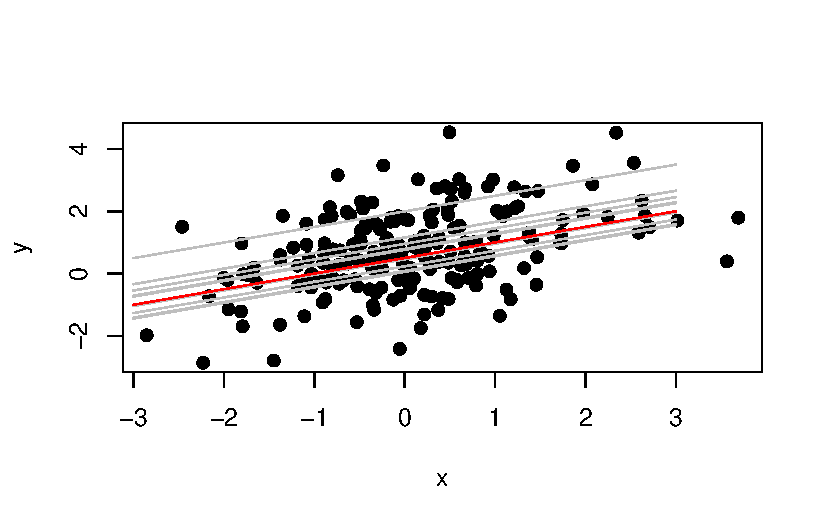
\includegraphics{varying_intercepts_varying_slopes_files/figure-pdf/unnamed-chunk-1-1.pdf}

Let's fit a varying intercepts model to this data.

\begin{Shaded}
\begin{Highlighting}[]
\FunctionTok{library}\NormalTok{(lme4)}
\FunctionTok{library}\NormalTok{(arm)}
\NormalTok{grp }\OtherTok{\textless{}{-}} \FunctionTok{as.numeric}\NormalTok{(group)}
\NormalTok{mod1 }\OtherTok{\textless{}{-}} \FunctionTok{lmer}\NormalTok{(y }\SpecialCharTok{\textasciitilde{}} \DecValTok{1} \SpecialCharTok{+}\NormalTok{ x }\SpecialCharTok{+}\NormalTok{ (}\DecValTok{1}\SpecialCharTok{|}\NormalTok{grp))}
\FunctionTok{display}\NormalTok{(mod1)}
\end{Highlighting}
\end{Shaded}

\begin{verbatim}
lmer(formula = y ~ 1 + x + (1 | grp))
            coef.est coef.se
(Intercept) 0.75     0.17   
x           0.45     0.07   

Error terms:
 Groups   Name        Std.Dev.
 grp      (Intercept) 0.48    
 Residual             1.08    
---
number of obs: 200, groups: grp, 10
AIC = 626.2, DIC = 607.7
deviance = 613.0 
\end{verbatim}

So the model has point estimates of \(\overline{\alpha} = .75 \pm .34\),
\(\beta = .45 \pm .14\), \(\sigma_y = 1.08\), \(\sigma_{\alpha} = .48\).
This all is pretty close to our simulated values.

\subsection{Intro to varying intercepts and varying
slopes}\label{intro-to-varying-intercepts-and-varying-slopes}

It would be nice if we could just add an independent model:
\(\beta_j \sim Normal(\overline{\beta}, \sigma_{\beta})\).
Unfortunately, we are not so lucky. We could do this if we expect
\(\alpha_j\) and \(\beta_j\) to be uncorrelated, but they will often be
correlated, so we need to account for this. In this case, we will use
the multi-variate normal distribution to model the coefficients. Deep
breaths, here we go:

\[
\begin{align*}
y_i &\sim Normal(\mu_i, \sigma_y)\\
\mu_i &= \alpha_{j[i]} + \beta_{j[i]} x_i\\
\begin{bmatrix} \alpha_j \\ \beta_j \end{bmatrix} &\sim MVN(\begin{bmatrix} \overline{\alpha}\\\overline{\beta}\end{bmatrix}, \Sigma)\\
\Sigma &= \begin{bmatrix} \sigma_{\alpha}^2 \space \space \rho\sigma_{\alpha}\sigma_{\beta} \\ \rho\sigma_{\alpha}\sigma_{\beta} \space  \space \sigma_{\beta}^2\end{bmatrix}
\end{align*}
\]

Always be simulatin'!. The big new thing here is that now the
coefficients are allowed to co-vary. The strength of this covariance is
controlled by \(\rho\), or the correlation. Let's simulate a bunch of
\(\alpha\)'s and \(\beta\)'s with different values of \(\rho\). Because
correlation is easier to understand than covariance and standard
deviations are easier to understand than variances, we will break down
the covariance matrix above into: \(\Sigma = SRS\), where \(S\) is a
diagonal matrix with the standard deviations of the coefficients on the
diagonal and 0's everywhere else, and \(R\) is a correlation matrix with
1's on the diagonal and correlations elsewhere:

\[
\Sigma = \begin{bmatrix} \sigma_{\alpha} \space 0 \\ 0 \space \sigma_{\beta} \end{bmatrix}\begin{bmatrix} 1 \space \rho\\ \rho \space 1 \end{bmatrix}\begin{bmatrix} \sigma_{\alpha} \space 0 \\ 0 \space \sigma_{\beta} \end{bmatrix}
\]

\begin{Shaded}
\begin{Highlighting}[]
\NormalTok{coef\_sims }\OtherTok{\textless{}{-}} \ControlFlowTok{function}\NormalTok{(rho)\{}
\NormalTok{  n }\OtherTok{\textless{}{-}} \DecValTok{1000}
\NormalTok{  a\_bar }\OtherTok{\textless{}{-}}\NormalTok{ .}\DecValTok{5}
\NormalTok{  b\_bar }\OtherTok{\textless{}{-}}\NormalTok{ .}\DecValTok{5}
\NormalTok{  sig\_a }\OtherTok{\textless{}{-}} \FloatTok{1.1}
\NormalTok{  sig\_b }\OtherTok{\textless{}{-}} \FloatTok{1.5}
\NormalTok{  rho }\OtherTok{\textless{}{-}}\NormalTok{ rho}
\NormalTok{  S }\OtherTok{\textless{}{-}} \FunctionTok{diag}\NormalTok{(}\FunctionTok{c}\NormalTok{(sig\_a, sig\_b))}
\NormalTok{  R }\OtherTok{\textless{}{-}} \FunctionTok{matrix}\NormalTok{(}\FunctionTok{c}\NormalTok{(}\DecValTok{1}\NormalTok{, rho, rho, }\DecValTok{1}\NormalTok{), }\AttributeTok{ncol =} \DecValTok{2}\NormalTok{)}
  
\NormalTok{  a\_b }\OtherTok{\textless{}{-}}\NormalTok{ MASS}\SpecialCharTok{::}\FunctionTok{mvrnorm}\NormalTok{(n, }\FunctionTok{c}\NormalTok{(a\_bar, b\_bar), S }\SpecialCharTok{\%*\%}\NormalTok{ R }\SpecialCharTok{\%*\%}\NormalTok{ S)}
  \FunctionTok{plot}\NormalTok{(a\_b[,}\DecValTok{1}\NormalTok{] }\SpecialCharTok{\textasciitilde{}}\NormalTok{ a\_b[,}\DecValTok{2}\NormalTok{])}
\NormalTok{\}}
\FunctionTok{coef\_sims}\NormalTok{(}\DecValTok{0}\NormalTok{)}
\end{Highlighting}
\end{Shaded}

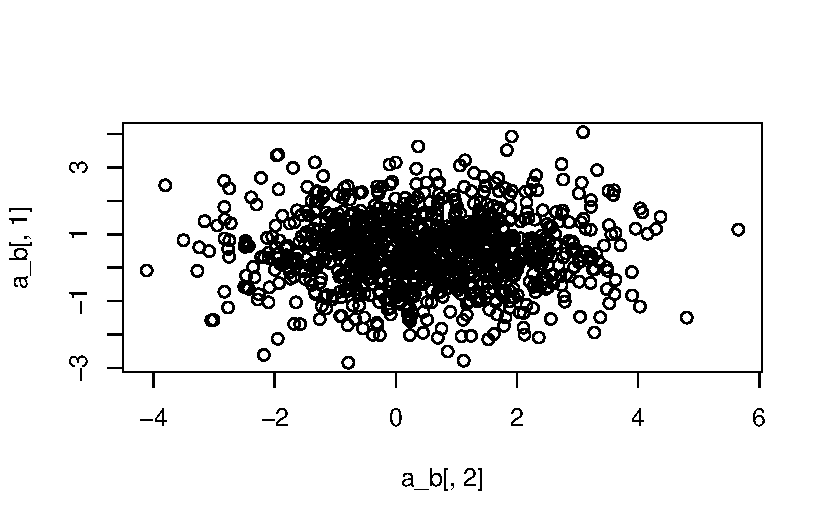
\includegraphics{varying_intercepts_varying_slopes_files/figure-pdf/unnamed-chunk-3-1.pdf}

\begin{Shaded}
\begin{Highlighting}[]
\FunctionTok{coef\_sims}\NormalTok{(.}\DecValTok{5}\NormalTok{)}
\end{Highlighting}
\end{Shaded}

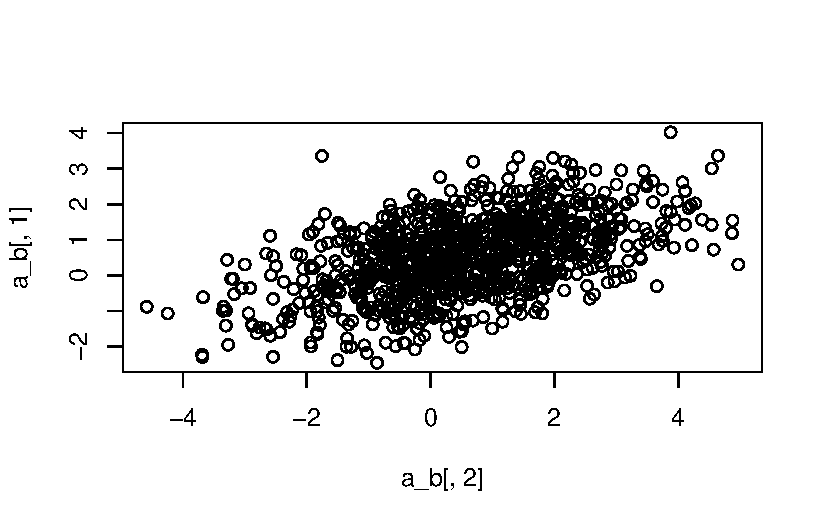
\includegraphics{varying_intercepts_varying_slopes_files/figure-pdf/unnamed-chunk-3-2.pdf}

\begin{Shaded}
\begin{Highlighting}[]
\FunctionTok{coef\_sims}\NormalTok{(.}\DecValTok{75}\NormalTok{)}
\end{Highlighting}
\end{Shaded}

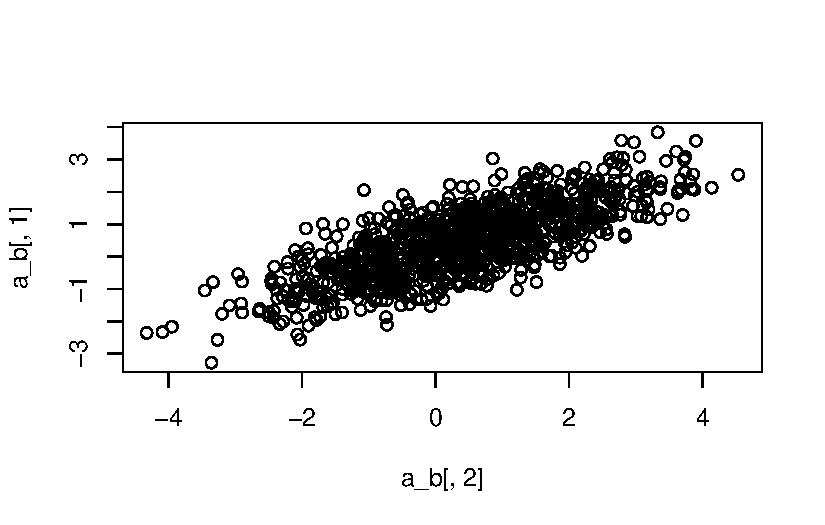
\includegraphics{varying_intercepts_varying_slopes_files/figure-pdf/unnamed-chunk-3-3.pdf}

\begin{Shaded}
\begin{Highlighting}[]
\FunctionTok{coef\_sims}\NormalTok{(}\SpecialCharTok{{-}}\NormalTok{.}\DecValTok{5}\NormalTok{)}
\end{Highlighting}
\end{Shaded}

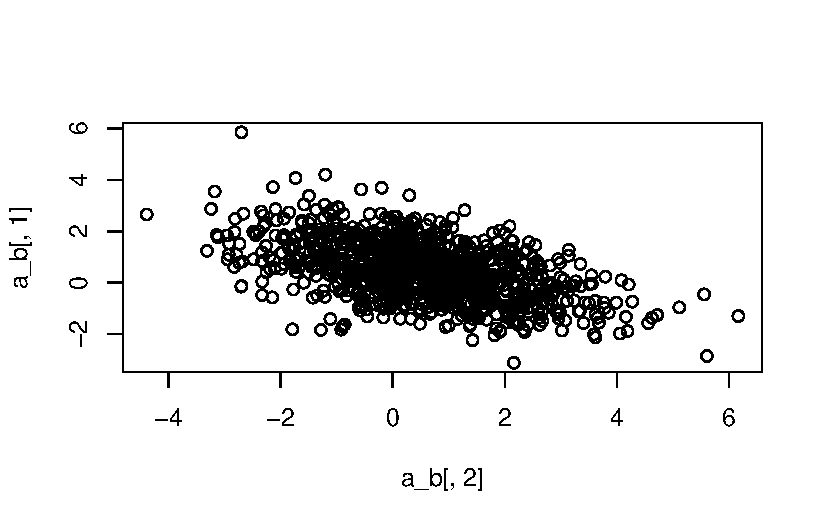
\includegraphics{varying_intercepts_varying_slopes_files/figure-pdf/unnamed-chunk-3-4.pdf}

\begin{Shaded}
\begin{Highlighting}[]
\FunctionTok{coef\_sims}\NormalTok{(}\SpecialCharTok{{-}}\NormalTok{.}\DecValTok{75}\NormalTok{)}
\FunctionTok{abline}\NormalTok{(}\AttributeTok{a =}\NormalTok{ .}\DecValTok{5} \SpecialCharTok{{-}}\NormalTok{ .}\DecValTok{5}\SpecialCharTok{*{-}}\NormalTok{.}\DecValTok{75}\SpecialCharTok{*}\FloatTok{1.1}\SpecialCharTok{/}\FloatTok{1.5}\NormalTok{, }\AttributeTok{b =} \SpecialCharTok{{-}}\NormalTok{.}\DecValTok{75}\SpecialCharTok{*}\FloatTok{1.1}\SpecialCharTok{*}\FloatTok{1.5}\SpecialCharTok{/}\NormalTok{(}\FloatTok{1.5}\SpecialCharTok{\^{}}\DecValTok{2}\NormalTok{), }\AttributeTok{col =} \StringTok{"blue"}\NormalTok{)}
\end{Highlighting}
\end{Shaded}

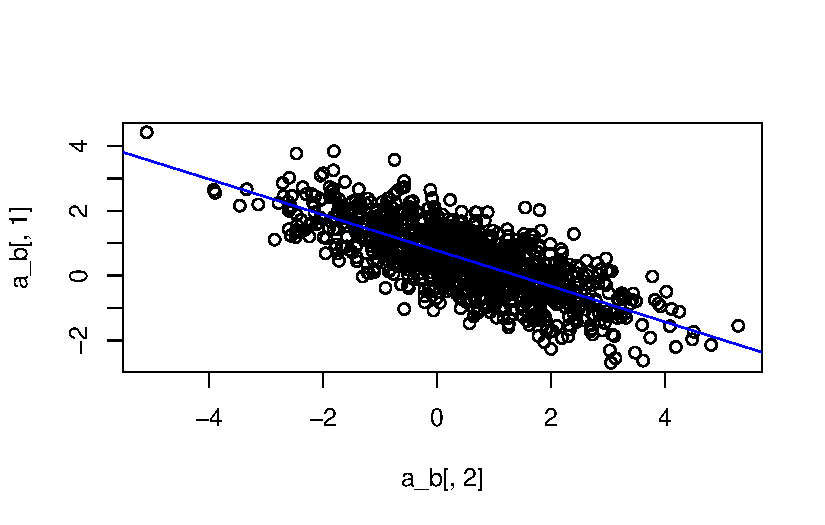
\includegraphics{varying_intercepts_varying_slopes_files/figure-pdf/unnamed-chunk-3-5.pdf}

\begin{Shaded}
\begin{Highlighting}[]
\FunctionTok{coef\_sims}\NormalTok{(}\DecValTok{1}\NormalTok{)}
\FunctionTok{abline}\NormalTok{(}\AttributeTok{a =}\NormalTok{ .}\DecValTok{5} \SpecialCharTok{{-}}\NormalTok{ .}\DecValTok{5}\SpecialCharTok{*}\FloatTok{1.1}\SpecialCharTok{/}\FloatTok{1.5}\NormalTok{, }\AttributeTok{b =} \DecValTok{1}\SpecialCharTok{*}\FloatTok{1.1}\SpecialCharTok{*}\FloatTok{1.5}\SpecialCharTok{/}\NormalTok{(}\FloatTok{1.5}\SpecialCharTok{\^{}}\DecValTok{2}\NormalTok{), }\AttributeTok{col =} \StringTok{"blue"}\NormalTok{)}
\end{Highlighting}
\end{Shaded}

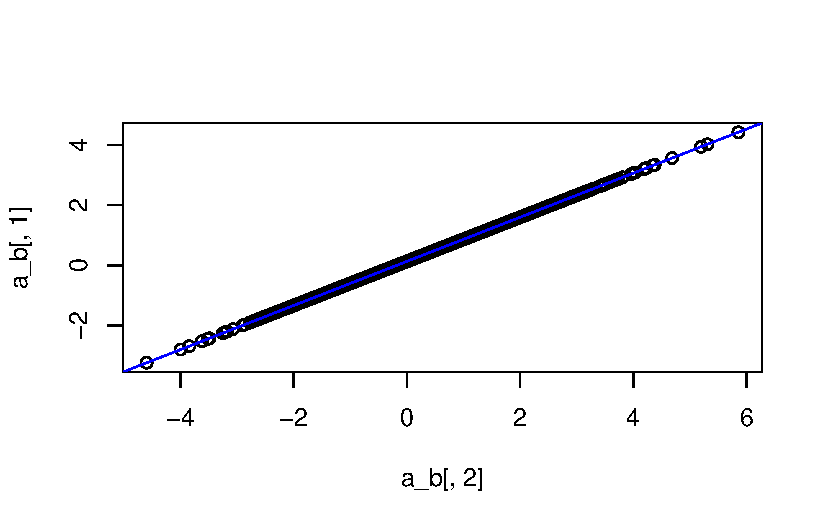
\includegraphics{varying_intercepts_varying_slopes_files/figure-pdf/unnamed-chunk-3-6.pdf}

So let's go ahead and simulate a varying slopes and varying intercepts
data generating process and fit it.

\begin{Shaded}
\begin{Highlighting}[]
\NormalTok{n }\OtherTok{\textless{}{-}} \DecValTok{200}
\NormalTok{a\_bar }\OtherTok{\textless{}{-}} \DecValTok{0}
\NormalTok{b\_bar }\OtherTok{\textless{}{-}}\NormalTok{ .}\DecValTok{5}
\NormalTok{sig\_a }\OtherTok{\textless{}{-}}\NormalTok{ .}\DecValTok{75}
\NormalTok{sig\_b }\OtherTok{\textless{}{-}} \FloatTok{1.1}
\NormalTok{sig\_y }\OtherTok{\textless{}{-}} \DecValTok{1}
\NormalTok{rho }\OtherTok{\textless{}{-}}\NormalTok{ .}\DecValTok{5}
\NormalTok{S }\OtherTok{\textless{}{-}} \FunctionTok{diag}\NormalTok{(}\FunctionTok{c}\NormalTok{(sig\_a, sig\_b))}
\NormalTok{R }\OtherTok{\textless{}{-}} \FunctionTok{matrix}\NormalTok{(}\FunctionTok{c}\NormalTok{(}\DecValTok{1}\NormalTok{, rho, rho, }\DecValTok{1}\NormalTok{), }\AttributeTok{ncol =} \DecValTok{2}\NormalTok{)}

\NormalTok{a\_b }\OtherTok{\textless{}{-}}\NormalTok{ MASS}\SpecialCharTok{::}\FunctionTok{mvrnorm}\NormalTok{(}\DecValTok{20}\NormalTok{, }\FunctionTok{c}\NormalTok{(a\_bar, b\_bar), S }\SpecialCharTok{\%*\%}\NormalTok{ R }\SpecialCharTok{\%*\%}\NormalTok{ S)}

\NormalTok{group }\OtherTok{\textless{}{-}} \FunctionTok{sample}\NormalTok{(}\DecValTok{1}\SpecialCharTok{:}\DecValTok{20}\NormalTok{, n, }\AttributeTok{replace =}\NormalTok{ T)}

\NormalTok{x }\OtherTok{\textless{}{-}} \FunctionTok{rnorm}\NormalTok{(n)}

\NormalTok{mu }\OtherTok{\textless{}{-}}\NormalTok{ a\_b[group, }\DecValTok{1}\NormalTok{] }\SpecialCharTok{+}\NormalTok{ a\_b[group, }\DecValTok{2}\NormalTok{] }\SpecialCharTok{*}\NormalTok{ x}

\NormalTok{y }\OtherTok{\textless{}{-}} \FunctionTok{rnorm}\NormalTok{(n, mu, sig\_y)}

\FunctionTok{plot}\NormalTok{(y }\SpecialCharTok{\textasciitilde{}}\NormalTok{ x, }\AttributeTok{pch =} \DecValTok{19}\NormalTok{)}
\end{Highlighting}
\end{Shaded}

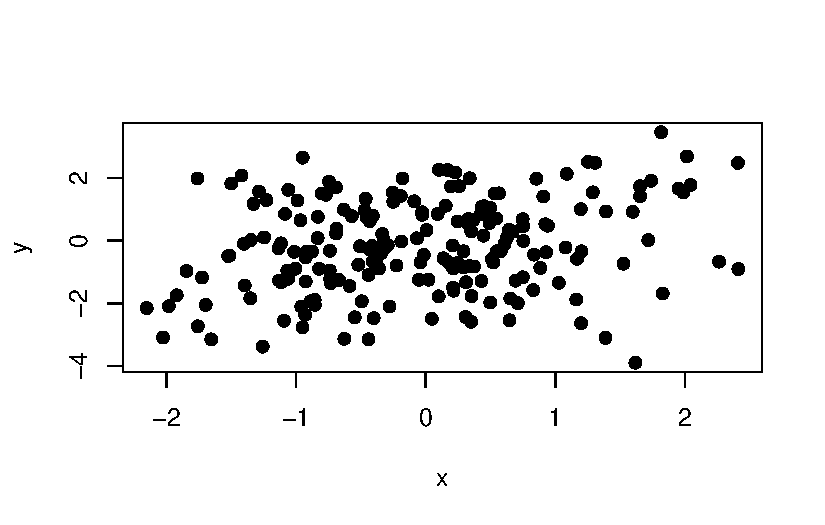
\includegraphics{varying_intercepts_varying_slopes_files/figure-pdf/unnamed-chunk-4-1.pdf}

Kinda hard to see what's going on, let's plot all the groups.

\begin{Shaded}
\begin{Highlighting}[]
\FunctionTok{library}\NormalTok{(tidyverse)}
\FunctionTok{data.frame}\NormalTok{(y, x, group) }\SpecialCharTok{\%\textgreater{}\%} 
  \FunctionTok{ggplot}\NormalTok{(}\FunctionTok{aes}\NormalTok{(}\AttributeTok{x =}\NormalTok{ x, }\AttributeTok{y =}\NormalTok{ y)) }\SpecialCharTok{+}
  \FunctionTok{geom\_point}\NormalTok{() }\SpecialCharTok{+}
  \FunctionTok{facet\_wrap}\NormalTok{(group }\SpecialCharTok{\textasciitilde{}}\NormalTok{ .)}
\end{Highlighting}
\end{Shaded}

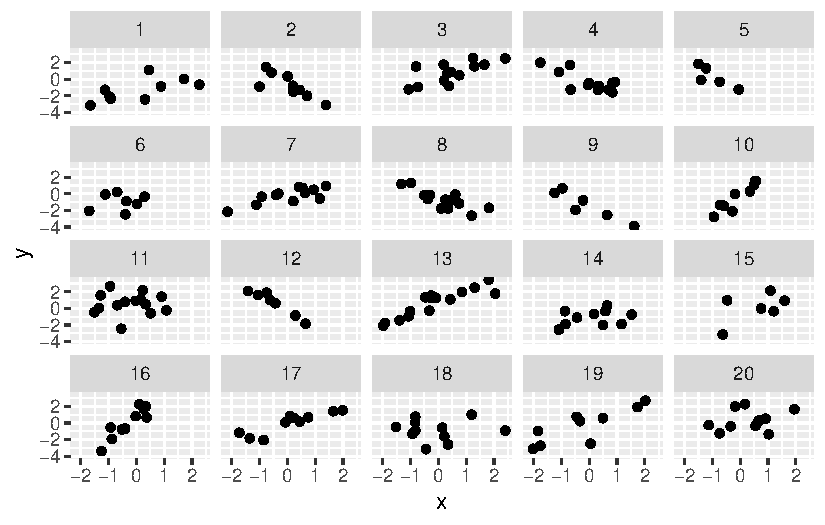
\includegraphics{varying_intercepts_varying_slopes_files/figure-pdf/unnamed-chunk-5-1.pdf}

Now let's fit the model with \texttt{lmer}.

\begin{Shaded}
\begin{Highlighting}[]
\NormalTok{grp }\OtherTok{\textless{}{-}} \FunctionTok{factor}\NormalTok{(group)}
\NormalTok{mod2 }\OtherTok{\textless{}{-}} \FunctionTok{lmer}\NormalTok{(y }\SpecialCharTok{\textasciitilde{}} \DecValTok{1} \SpecialCharTok{+}\NormalTok{ x }\SpecialCharTok{+}\NormalTok{ (}\DecValTok{1} \SpecialCharTok{+}\NormalTok{ x}\SpecialCharTok{|}\NormalTok{grp))}
\FunctionTok{display}\NormalTok{(mod2)}
\end{Highlighting}
\end{Shaded}

\begin{verbatim}
lmer(formula = y ~ 1 + x + (1 + x | grp))
            coef.est coef.se
(Intercept) -0.30     0.16  
x            0.22     0.28  

Error terms:
 Groups   Name        Std.Dev. Corr 
 grp      (Intercept) 0.61          
          x           1.18     0.56 
 Residual             0.97          
---
number of obs: 200, groups: grp, 20
AIC = 645.2, DIC = 627.4
deviance = 630.3 
\end{verbatim}

\begin{Shaded}
\begin{Highlighting}[]
\NormalTok{fits }\OtherTok{\textless{}{-}} \FunctionTok{data.frame}\NormalTok{(}\AttributeTok{group =} \DecValTok{1}\SpecialCharTok{:}\DecValTok{20}\NormalTok{, }\AttributeTok{a =} \FunctionTok{coef}\NormalTok{(mod2)}\SpecialCharTok{$}\NormalTok{grp[,}\DecValTok{1}\NormalTok{], }\AttributeTok{b =} \FunctionTok{coef}\NormalTok{(mod2)}\SpecialCharTok{$}\NormalTok{grp[,}\DecValTok{2}\NormalTok{])}
\end{Highlighting}
\end{Shaded}

Let's plot the mean fits on the data

\begin{Shaded}
\begin{Highlighting}[]
\FunctionTok{data.frame}\NormalTok{(y, x, group) }\SpecialCharTok{\%\textgreater{}\%} 
  \FunctionTok{ggplot}\NormalTok{(}\FunctionTok{aes}\NormalTok{(}\AttributeTok{x =}\NormalTok{ x, }\AttributeTok{y =}\NormalTok{ y)) }\SpecialCharTok{+}
  \FunctionTok{geom\_point}\NormalTok{() }\SpecialCharTok{+}
  \FunctionTok{facet\_wrap}\NormalTok{(group }\SpecialCharTok{\textasciitilde{}}\NormalTok{ .) }\SpecialCharTok{+}
  \FunctionTok{geom\_vline}\NormalTok{(}\AttributeTok{xintercept =} \DecValTok{0}\NormalTok{, }\AttributeTok{color =} \StringTok{"grey"}\NormalTok{) }\SpecialCharTok{+}
  \FunctionTok{geom\_hline}\NormalTok{(}\AttributeTok{yintercept =} \DecValTok{0}\NormalTok{, }\AttributeTok{color =} \StringTok{"grey"}\NormalTok{) }\SpecialCharTok{+}
  \FunctionTok{geom\_abline}\NormalTok{(}\AttributeTok{data =}\NormalTok{ fits, }\FunctionTok{aes}\NormalTok{(}\AttributeTok{slope =}\NormalTok{ b, }\AttributeTok{intercept =}\NormalTok{ a))}
\end{Highlighting}
\end{Shaded}

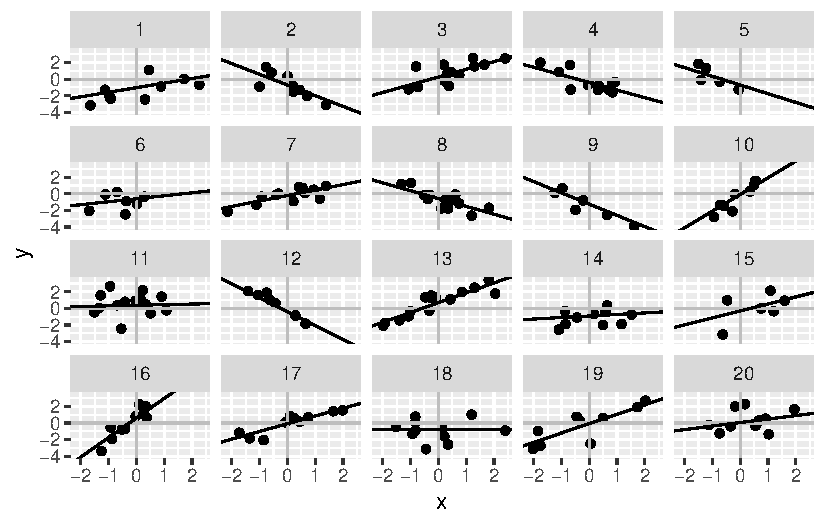
\includegraphics{varying_intercepts_varying_slopes_files/figure-pdf/unnamed-chunk-7-1.pdf}

\subsection{Adding Group Level
Predictors}\label{adding-group-level-predictors}

Let's load in the plant growth data to play around with some real data.
Let's plot it to see what it looks like. There are many things that we
might be interested about in this data set. Let's start off by trying to
estimate growth rates. In this case, growth rate will be the regression
coefficient on age.

\begin{Shaded}
\begin{Highlighting}[]
\FunctionTok{library}\NormalTok{(here)}
\NormalTok{growth\_dat }\OtherTok{\textless{}{-}} \FunctionTok{read.csv}\NormalTok{(}\FunctionTok{here}\NormalTok{(}\StringTok{"data/week\_10/plant\_growth.csv"}\NormalTok{))}
\FunctionTok{head}\NormalTok{(growth\_dat)}
\end{Highlighting}
\end{Shaded}

\begin{verbatim}
   id   seed_size   size age
1 1_1  0.04398394  1.915   1
2 1_1  0.04398394  4.016   3
3 1_1  0.04398394  7.821   6
4 1_2 -0.01040480  3.133   1
5 1_2 -0.01040480  5.999   3
6 1_2 -0.01040480 15.602   6
\end{verbatim}

\begin{Shaded}
\begin{Highlighting}[]
\NormalTok{growth\_dat }\SpecialCharTok{\%\textgreater{}\%} 
  \FunctionTok{ggplot}\NormalTok{(}\FunctionTok{aes}\NormalTok{(}\AttributeTok{x =}\NormalTok{ age, }\AttributeTok{y =}\NormalTok{ size)) }\SpecialCharTok{+}
  \FunctionTok{geom\_point}\NormalTok{()}
\end{Highlighting}
\end{Shaded}

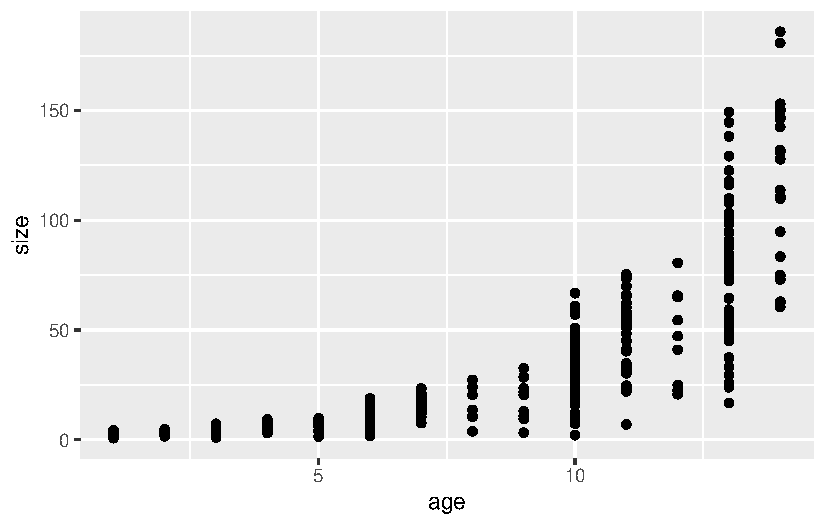
\includegraphics{varying_intercepts_varying_slopes_files/figure-pdf/unnamed-chunk-8-1.pdf}

Looks like exponential growth. We could probably use a log-normal GLMM,
but let's transform it for fun.

\begin{Shaded}
\begin{Highlighting}[]
\NormalTok{growth\_dat}\SpecialCharTok{$}\NormalTok{l\_size }\OtherTok{\textless{}{-}} \FunctionTok{log}\NormalTok{(growth\_dat}\SpecialCharTok{$}\NormalTok{size)}

\NormalTok{growth\_dat }\SpecialCharTok{\%\textgreater{}\%} 
  \FunctionTok{ggplot}\NormalTok{(}\FunctionTok{aes}\NormalTok{(}\AttributeTok{x =}\NormalTok{ age, }\AttributeTok{y =}\NormalTok{ l\_size)) }\SpecialCharTok{+}
  \FunctionTok{geom\_point}\NormalTok{()}
\end{Highlighting}
\end{Shaded}

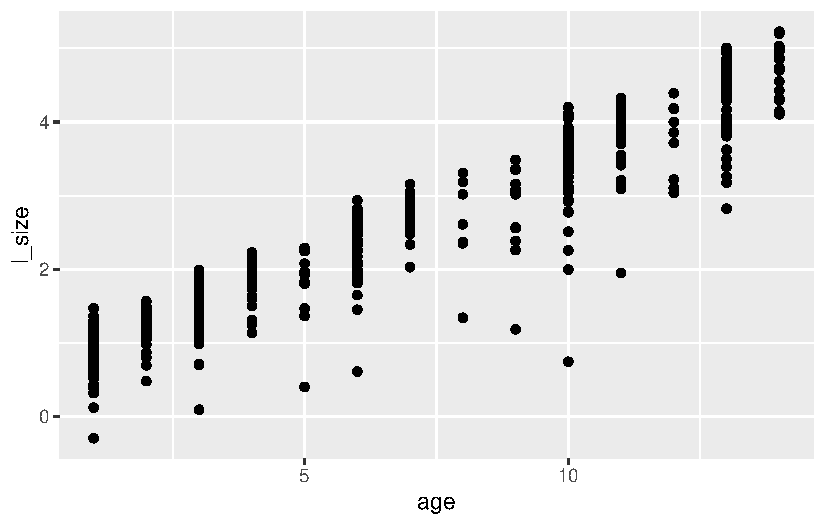
\includegraphics{varying_intercepts_varying_slopes_files/figure-pdf/unnamed-chunk-9-1.pdf}

It looks nice and linear now! So let's do some modeling. It is probably
a bad idea to completely pool this data since multiple measures were
taken for each individual. So we will use a multilevel model (partial
pooling) to get at the variation between individuals. Let's fit no-pool
model as well and compare the intercepts

\begin{Shaded}
\begin{Highlighting}[]
\NormalTok{growth\_dat}\SpecialCharTok{$}\NormalTok{id }\OtherTok{\textless{}{-}} \FunctionTok{factor}\NormalTok{(growth\_dat}\SpecialCharTok{$}\NormalTok{id)}
\NormalTok{mod\_p\_pool }\OtherTok{\textless{}{-}} \FunctionTok{lmer}\NormalTok{(l\_size }\SpecialCharTok{\textasciitilde{}} \DecValTok{1} \SpecialCharTok{+}\NormalTok{ age }\SpecialCharTok{+}\NormalTok{ (}\DecValTok{1} \SpecialCharTok{+}\NormalTok{ age}\SpecialCharTok{|}\NormalTok{id), }\AttributeTok{data =}\NormalTok{ growth\_dat)}
\NormalTok{mod\_no\_pool }\OtherTok{\textless{}{-}} \FunctionTok{lm}\NormalTok{(l\_size }\SpecialCharTok{\textasciitilde{}} \SpecialCharTok{{-}}\DecValTok{1} \SpecialCharTok{+}\NormalTok{ age }\SpecialCharTok{+}\NormalTok{ id }\SpecialCharTok{+}\NormalTok{ id}\SpecialCharTok{*}\NormalTok{age, }\AttributeTok{data =}\NormalTok{ growth\_dat)}
\NormalTok{fit\_no\_pool }\OtherTok{\textless{}{-}} \FunctionTok{as.numeric}\NormalTok{(}\FunctionTok{coef}\NormalTok{(mod\_no\_pool)[}\DecValTok{2}\SpecialCharTok{:}\DecValTok{116}\NormalTok{])}
\NormalTok{fit\_p\_pool }\OtherTok{\textless{}{-}} \FunctionTok{coef}\NormalTok{(mod\_p\_pool)}\SpecialCharTok{$}\NormalTok{id[,}\DecValTok{1}\NormalTok{]}
\FunctionTok{plot}\NormalTok{(fit\_no\_pool, }\AttributeTok{pch =} \DecValTok{19}\NormalTok{)}
\FunctionTok{points}\NormalTok{(fit\_p\_pool, }\AttributeTok{col =} \StringTok{"blue"}\NormalTok{, }\AttributeTok{ylab =} \StringTok{"Intercept"}\NormalTok{, }\AttributeTok{pch =} \DecValTok{19}\NormalTok{)}
\FunctionTok{abline}\NormalTok{(}\AttributeTok{h =} \FunctionTok{fixef}\NormalTok{(mod\_p\_pool)[}\DecValTok{1}\NormalTok{])}
\end{Highlighting}
\end{Shaded}

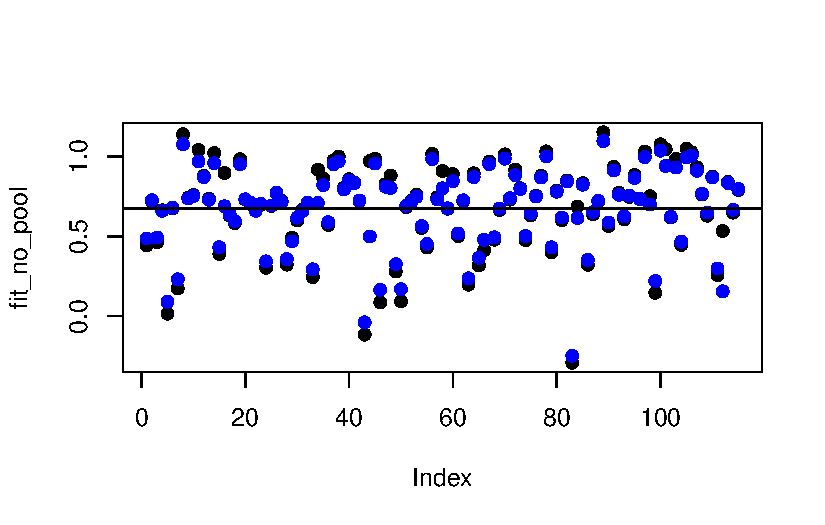
\includegraphics{varying_intercepts_varying_slopes_files/figure-pdf/unnamed-chunk-10-1.pdf}

Notice how, in general, the further the group intercepts get from the
mean, the more the partially pooled estimate is shrunk toward the mean!

\subsubsection{Adding a group level predictor to the
intercept}\label{adding-a-group-level-predictor-to-the-intercept}

So this is doing what we want, shrinking the intercepts toward the group
mean to help overfitting and use as much information as we can
reasonably use. But there is a variable we haven't considered yet. Seed
size is likely a major factor in the size of a seedling at time 0
(i.e.~the intercept). Let's try a varying intercepts model where the
intercept is a function of seed size. We want a model that looks like:

\[
\begin{align*}
size_{i} &\sim Normal(\mu_{i}, \sigma_{size})\\
\mu_i &= \alpha_{j[i]} + rate\times age_i\\
\alpha_{j} &\sim Normal(\overline{\alpha} + \gamma_{\alpha} \times seedsize_{j}, \sigma_{\alpha})
\end{align*}
\]

How do we get this into \texttt{lmer} though? Well, if we remember that
this form of the model of \(\alpha_j\) is just a re-writing of the form:

\[
\begin{align*}
\alpha_j &= \overline{\alpha} + \gamma_{\alpha} \times seedsize_j + \eta_j\\
\eta_j &\sim Nomral(0, \sigma_{\alpha})
\end{align*}
\] We can plug this definition of \(\alpha_j\) into the level one
equation:

\[
\begin{align*}
\mu_i &= (\overline{\alpha} + \gamma_{\alpha} \times seedsize_j + \eta_j) + rate\times age_i\\
\end{align*}
\] So, in \texttt{lmer} it becomes:
\texttt{lmer(l\_size\ \textasciitilde{}\ 1\ +\ seed\_size\ +\ age\ +\ (1\textbar{}id))}.
Let's try it out.

\begin{Shaded}
\begin{Highlighting}[]
\NormalTok{mod\_seed\_int }\OtherTok{\textless{}{-}} \FunctionTok{lmer}\NormalTok{(l\_size }\SpecialCharTok{\textasciitilde{}} \DecValTok{1} \SpecialCharTok{+}\NormalTok{ seed\_size }\SpecialCharTok{+}\NormalTok{ age }\SpecialCharTok{+}\NormalTok{ (}\DecValTok{1}\SpecialCharTok{|}\NormalTok{id), }\AttributeTok{data =}\NormalTok{ growth\_dat)}
\FunctionTok{display}\NormalTok{(mod\_seed\_int)}
\end{Highlighting}
\end{Shaded}

\begin{verbatim}
lmer(formula = l_size ~ 1 + seed_size + age + (1 | id), data = growth_dat)
            coef.est coef.se
(Intercept) 0.63     0.04   
seed_size   0.07     0.03   
age         0.28     0.00   

Error terms:
 Groups   Name        Std.Dev.
 id       (Intercept) 0.36    
 Residual             0.22    
---
number of obs: 562, groups: id, 115
AIC = 203.8, DIC = 153.2
deviance = 173.5 
\end{verbatim}

Let's plot the model for the group level intercepts! This might take
some \textbf{wrangling}:

\begin{Shaded}
\begin{Highlighting}[]
\NormalTok{seed\_size }\OtherTok{\textless{}{-}} \FunctionTok{unique}\NormalTok{(growth\_dat[,}\FunctionTok{c}\NormalTok{(}\StringTok{"id"}\NormalTok{, }\StringTok{"seed\_size"}\NormalTok{)])}
\NormalTok{sims }\OtherTok{\textless{}{-}} \FunctionTok{sim}\NormalTok{(mod\_seed\_int, }\DecValTok{1000}\NormalTok{)}
\NormalTok{rans }\OtherTok{\textless{}{-}} \FunctionTok{t}\NormalTok{(sims}\SpecialCharTok{@}\NormalTok{ranef}\SpecialCharTok{$}\NormalTok{id[,,}\DecValTok{1}\NormalTok{])}
\NormalTok{ints }\OtherTok{\textless{}{-}} \FunctionTok{matrix}\NormalTok{(}\AttributeTok{nrow =} \DecValTok{115}\NormalTok{, }\AttributeTok{ncol =} \DecValTok{1000}\NormalTok{)}
\ControlFlowTok{for}\NormalTok{(i }\ControlFlowTok{in} \DecValTok{1}\SpecialCharTok{:}\DecValTok{1000}\NormalTok{)\{}
\NormalTok{  ints[,i] }\OtherTok{\textless{}{-}} \FunctionTok{exp}\NormalTok{(rans[,i] }\SpecialCharTok{+}\NormalTok{ sims}\SpecialCharTok{@}\NormalTok{fixef[i,}\DecValTok{1}\NormalTok{] }\SpecialCharTok{+}\NormalTok{ seed\_size}\SpecialCharTok{$}\NormalTok{seed\_size }\SpecialCharTok{*}\NormalTok{ sims}\SpecialCharTok{@}\NormalTok{fixef[i,}\DecValTok{2}\NormalTok{])}
\NormalTok{\}}

\NormalTok{ints }\OtherTok{\textless{}{-}} \FunctionTok{data.frame}\NormalTok{(ints)}
\NormalTok{z }\OtherTok{\textless{}{-}} \FunctionTok{data.frame}\NormalTok{(}\AttributeTok{mu =} \FunctionTok{apply}\NormalTok{(ints, }\DecValTok{1}\NormalTok{, mean), }\AttributeTok{upr =} \FunctionTok{apply}\NormalTok{(ints, }\DecValTok{1}\NormalTok{, quantile, .}\DecValTok{975}\NormalTok{), }\AttributeTok{lwr =} \FunctionTok{apply}\NormalTok{(ints, }\DecValTok{1}\NormalTok{, quantile, .}\DecValTok{025}\NormalTok{), }\AttributeTok{seed\_size =}\NormalTok{ seed\_size}\SpecialCharTok{$}\NormalTok{seed\_size, }\AttributeTok{id =}\NormalTok{ seed\_size}\SpecialCharTok{$}\NormalTok{id)}

\NormalTok{seed\_pred }\OtherTok{\textless{}{-}} \FunctionTok{seq}\NormalTok{(}\SpecialCharTok{{-}}\DecValTok{3}\NormalTok{,}\DecValTok{3}\NormalTok{,}\AttributeTok{l =} \DecValTok{100}\NormalTok{)}
\NormalTok{int\_pred }\OtherTok{\textless{}{-}}\NormalTok{ int\_upr }\OtherTok{\textless{}{-}}\NormalTok{ int\_lwr }\OtherTok{\textless{}{-}} \FunctionTok{c}\NormalTok{()}
\ControlFlowTok{for}\NormalTok{(i }\ControlFlowTok{in} \DecValTok{1}\SpecialCharTok{:}\DecValTok{100}\NormalTok{)\{}
\NormalTok{  temp }\OtherTok{\textless{}{-}}\NormalTok{ sims}\SpecialCharTok{@}\NormalTok{fixef[,}\DecValTok{1}\NormalTok{] }\SpecialCharTok{+}\NormalTok{ sims}\SpecialCharTok{@}\NormalTok{fixef[,}\DecValTok{2}\NormalTok{] }\SpecialCharTok{*}\NormalTok{ seed\_pred[i]}
\NormalTok{  int\_pred[i] }\OtherTok{\textless{}{-}} \FunctionTok{exp}\NormalTok{(}\FunctionTok{mean}\NormalTok{(temp))}
\NormalTok{  int\_upr[i] }\OtherTok{\textless{}{-}} \FunctionTok{exp}\NormalTok{(}\FunctionTok{quantile}\NormalTok{(temp, .}\DecValTok{975}\NormalTok{))}
\NormalTok{  int\_lwr[i] }\OtherTok{\textless{}{-}} \FunctionTok{exp}\NormalTok{(}\FunctionTok{quantile}\NormalTok{(temp, .}\DecValTok{025}\NormalTok{))}
\NormalTok{\}}

\FunctionTok{data.frame}\NormalTok{(seed\_pred, int\_pred, int\_upr, int\_lwr) }\SpecialCharTok{\%\textgreater{}\%} 
  \FunctionTok{ggplot}\NormalTok{(}\FunctionTok{aes}\NormalTok{(}\AttributeTok{x =}\NormalTok{ seed\_pred, }\AttributeTok{y =}\NormalTok{ int\_pred)) }\SpecialCharTok{+}
  \FunctionTok{geom\_line}\NormalTok{() }\SpecialCharTok{+}
  \FunctionTok{geom\_ribbon}\NormalTok{(}\FunctionTok{aes}\NormalTok{(}\AttributeTok{x =}\NormalTok{ seed\_pred, }\AttributeTok{ymax =}\NormalTok{ int\_upr, }\AttributeTok{ymin =}\NormalTok{ int\_lwr), }\AttributeTok{alpha =}\NormalTok{ .}\DecValTok{25}\NormalTok{) }\SpecialCharTok{+}
  \FunctionTok{geom\_point}\NormalTok{(}\AttributeTok{data =}\NormalTok{ z, }\FunctionTok{aes}\NormalTok{(}\AttributeTok{x =}\NormalTok{ seed\_size, }\AttributeTok{y =}\NormalTok{ mu)) }\SpecialCharTok{+}
  \FunctionTok{geom\_errorbar}\NormalTok{(}\AttributeTok{data =}\NormalTok{ z, }\FunctionTok{aes}\NormalTok{(}\AttributeTok{x =}\NormalTok{ seed\_size, }\AttributeTok{ymax =}\NormalTok{ upr, }\AttributeTok{ymin =}\NormalTok{ lwr), }\AttributeTok{inherit.aes =}\NormalTok{ F,}
                \AttributeTok{width =} \DecValTok{0}\NormalTok{)}
\end{Highlighting}
\end{Shaded}

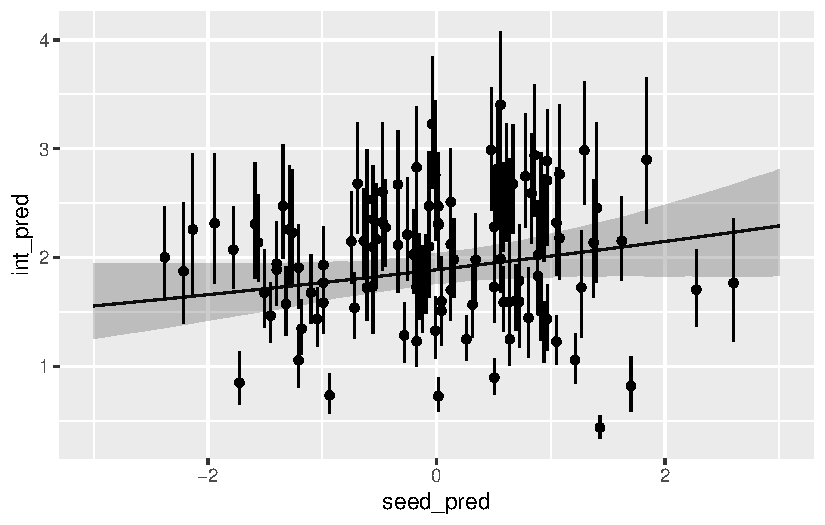
\includegraphics{varying_intercepts_varying_slopes_files/figure-pdf/unnamed-chunk-12-1.pdf}

\subsubsection{Adding group level predictors to the slope: or, group
level predictors as
interactions.}\label{adding-group-level-predictors-to-the-slope-or-group-level-predictors-as-interactions.}

How to add group level predictors to the slope using \texttt{lmer} is
not intuitive--to me at least. But I think it is helpful to view adding
these predictors as creating an interaction between the group level
predictor, and the individual level predictor. This helps me think about
statistical interactions. I.E. the ``main effect'' is the value of the
slope on the individual level predictor when the group level predictor =
0; the slope on the interaction adjusts the slope for each group. Let's
build this up.

\[
\begin{align*}
y_i &\sim Normal(\mu_i, \sigma_y)\\
\mu_i &= \alpha_{j[i]} + \beta_{j[i]} x_i\\
\begin{bmatrix} \alpha_j \\ \beta_j \end{bmatrix} &= MVNormal(\begin{bmatrix} \overline{\alpha} + \gamma_{\alpha} u_j \\ \overline{\beta} + \gamma_{\beta} u_j \end{bmatrix}, \Sigma)
\end{align*}
\]

So, now we have our individual level predictor, \(x\) and our group
level predictor, \(u\). To see how we can use \texttt{lmer} to do this,
we can stick our linear models for the intercept and slope into the
single level model:

\[
\begin{align*}
\mu_i &= \alpha_{j[i]} + \beta_{j[i]} x_i\\
&= (\overline{\alpha} + \gamma_{\alpha} u_{i[j]}) + (\overline{\beta} + \gamma_{\beta} u_{j[i]}) x_i\\
&= \overline{\alpha} + \gamma_{\alpha} u_{j[i]} + \overline{\beta} x_i + \gamma_{\beta} u_{j[i]}x_i
\end{align*}
\]

This gives us the formula we can use:
\texttt{lmer(y\ \textasciitilde{}\ 1\ +\ u\ +\ x\ +\ u*x\ +\ (1\ +\ x\textbar{}group))}.
Pretty cool! Let's fit this model:

\begin{Shaded}
\begin{Highlighting}[]
\NormalTok{mod\_var\_ints\_slopes }\OtherTok{\textless{}{-}} \FunctionTok{lmer}\NormalTok{(l\_size }\SpecialCharTok{\textasciitilde{}} \DecValTok{1} \SpecialCharTok{+}\NormalTok{ seed\_size }\SpecialCharTok{+}\NormalTok{ age }\SpecialCharTok{+}\NormalTok{ seed\_size}\SpecialCharTok{*}\NormalTok{age }\SpecialCharTok{+}\NormalTok{ (}\DecValTok{1} \SpecialCharTok{+}\NormalTok{ age}\SpecialCharTok{|}\NormalTok{id), }\AttributeTok{data =}\NormalTok{ growth\_dat)}
\FunctionTok{display}\NormalTok{(mod\_var\_ints\_slopes)}
\end{Highlighting}
\end{Shaded}

\begin{verbatim}
lmer(formula = l_size ~ 1 + seed_size + age + seed_size * age + 
    (1 + age | id), data = growth_dat)
              coef.est coef.se
(Intercept)   0.67     0.02   
seed_size     0.07     0.02   
age           0.27     0.00   
seed_size:age 0.00     0.00   

Error terms:
 Groups   Name        Std.Dev. Corr 
 id       (Intercept) 0.25          
          age         0.05     0.07 
 Residual             0.11          
---
number of obs: 562, groups: id, 115
AIC = -150, DIC = -223.7
deviance = -194.9 
\end{verbatim}

Let's sort out this output in terms of our varying intercepts, varying
slopes model with predictors. First a reminder of the model: \[
\begin{align*}
y_i &\sim Normal(\mu_i, \sigma_y)\\
\mu_i &= \alpha_{j[i]} + \beta_{j[i]} x_i\\
\begin{bmatrix} \alpha_j \\ \beta_j \end{bmatrix} &\sim MVN(\begin{bmatrix} \overline{\alpha} + \gamma_{\alpha} u_j \\ \overline{\beta} + \gamma_{\beta} u_j\end{bmatrix}, \Sigma)\\
\Sigma &= \begin{bmatrix} \sigma_{\alpha}^2 \space \space \rho\sigma_{\alpha}\sigma_{\beta} \\ \rho\sigma_{\alpha}\sigma_{\beta} \space  \space \sigma_{\beta}^2\end{bmatrix}
\end{align*}
\] Let's fill it in with our model output:

\[
\begin{align*}
\log(size_i) &\sim Normal(\space\mu_i,\space .11)\\
\mu_i &= \alpha_{j[i]} + \beta_{j[i]} x_i\\
\begin{bmatrix} \alpha_j \\ \beta_j \end{bmatrix} &\sim MVN(\begin{bmatrix} .67 + .07 \times seedsize_j \\ .27 + 0\times seedsize_j\end{bmatrix}, \Sigma)\\
\Sigma &= \begin{bmatrix} .25^2 \space \space \space .07\times .25\times .05 \\ .07\times .25\times .05 \space \space  \space .05^2\end{bmatrix}
\end{align*}
\]

And that's our multilevel model. We have slopes and intercepts that vary
by individual plant and we have group level predictors that let us
potentially get better resolution on what drives variation between
groups, which is something that we can't do without partial pooling!



\end{document}
